% !TEX TS-program = knitr
\documentclass[handout]{beamer}\usepackage[]{graphicx}\usepackage[]{color}
% maxwidth is the original width if it is less than linewidth
% otherwise use linewidth (to make sure the graphics do not exceed the margin)
\makeatletter
\def\maxwidth{ %
  \ifdim\Gin@nat@width>\linewidth
    \linewidth
  \else
    \Gin@nat@width
  \fi
}
\makeatother

\definecolor{fgcolor}{rgb}{0.345, 0.345, 0.345}
\newcommand{\hlnum}[1]{\textcolor[rgb]{0.686,0.059,0.569}{#1}}%
\newcommand{\hlstr}[1]{\textcolor[rgb]{0.192,0.494,0.8}{#1}}%
\newcommand{\hlcom}[1]{\textcolor[rgb]{0.678,0.584,0.686}{\textit{#1}}}%
\newcommand{\hlopt}[1]{\textcolor[rgb]{0,0,0}{#1}}%
\newcommand{\hlstd}[1]{\textcolor[rgb]{0.345,0.345,0.345}{#1}}%
\newcommand{\hlkwa}[1]{\textcolor[rgb]{0.161,0.373,0.58}{\textbf{#1}}}%
\newcommand{\hlkwb}[1]{\textcolor[rgb]{0.69,0.353,0.396}{#1}}%
\newcommand{\hlkwc}[1]{\textcolor[rgb]{0.333,0.667,0.333}{#1}}%
\newcommand{\hlkwd}[1]{\textcolor[rgb]{0.737,0.353,0.396}{\textbf{#1}}}%
\let\hlipl\hlkwb

\usepackage{framed}
\makeatletter
\newenvironment{kframe}{%
 \def\at@end@of@kframe{}%
 \ifinner\ifhmode%
  \def\at@end@of@kframe{\end{minipage}}%
  \begin{minipage}{\columnwidth}%
 \fi\fi%
 \def\FrameCommand##1{\hskip\@totalleftmargin \hskip-\fboxsep
 \colorbox{shadecolor}{##1}\hskip-\fboxsep
     % There is no \\@totalrightmargin, so:
     \hskip-\linewidth \hskip-\@totalleftmargin \hskip\columnwidth}%
 \MakeFramed {\advance\hsize-\width
   \@totalleftmargin\z@ \linewidth\hsize
   \@setminipage}}%
 {\par\unskip\endMakeFramed%
 \at@end@of@kframe}
\makeatother

\definecolor{shadecolor}{rgb}{.97, .97, .97}
\definecolor{messagecolor}{rgb}{0, 0, 0}
\definecolor{warningcolor}{rgb}{1, 0, 1}
\definecolor{errorcolor}{rgb}{1, 0, 0}
\newenvironment{knitrout}{}{} % an empty environment to be redefined in TeX

\usepackage{alltt}
\newcommand{\answers}{1}

\usetheme{Marburg}
\setbeamertemplate{navigation symbols}{} 
\setbeamertemplate{footline}
{
  \leavevmode%
  \hbox{%
  \begin{beamercolorbox}[wd=.333333\paperwidth,ht=2.25ex,dp=1ex,center]{author in head/foot}%
    \usebeamerfont{author in head/foot} $\ $ \insertshortauthor%~~\beamer@ifempty{\insertshortinstitute}{}{(\insertshortinstitute)}
  \end{beamercolorbox}%
  \begin{beamercolorbox}[wd=.333333\paperwidth,ht=2.25ex,dp=1ex,center]{title in head/foot}%
    \usebeamerfont{title in head/foot} \insertinstitute
  \end{beamercolorbox}%
  \begin{beamercolorbox}[wd=.333333\paperwidth,ht=2.25ex,dp=1ex,right]{date in head/foot}%
    \usebeamerfont{date in head/foot}\insertshortdate{}\hspace*{2em}
    \insertframenumber{} / \inserttotalframenumber\hspace*{2ex} 
  \end{beamercolorbox}}%
  \vskip0pt%
}

\usepackage{amsmath}
\usepackage{caption}
\usepackage{color}
\usepackage{enumerate}
\usepackage{listings}
\usepackage{hyperref}
\usepackage{mathrsfs}
\usepackage{natbib}
\usepackage{url}

\providecommand{\all}{\ \forall \ }
\providecommand{\bs}{\backslash}
\providecommand{\e}{\varepsilon}
\providecommand{\E}{\ \exists \ }
\providecommand{\lm}[2]{\lim_{#1 \rightarrow #2}}
\providecommand{\m}[1]{\mathbb{#1}}
\providecommand{\nv}{{}^{-1}}
\providecommand{\ov}[1]{\overline{#1}}
\providecommand{\p}{\newpage}
\providecommand{\q}{$\quad$ \newline}
\providecommand{\rt}{\rightarrow}
\providecommand{\Rt}{\Rightarrow}
\providecommand{\vc}[1]{\boldsymbol{#1}}
\providecommand{\wh}[1]{\widehat{#1}}

\hypersetup{colorlinks,linkcolor=,urlcolor=blue}
\numberwithin{equation}{section}

\definecolor{dkgreen}{rgb}{0,0.6,0}
\definecolor{gray}{rgb}{0.5,0.5,0.5}
\definecolor{mauve}{rgb}{0.58,0,0.82}

\lstset{ 
  language=C,                % the language of the code
  basicstyle= \footnotesize,           % the size of the fonts that are used for the code
  numberstyle= \tiny \color{white},  % the style that is used for the line-numbers
  stepnumber=2,                   % the step between two line-numbers. 
  numbersep=5pt,                  % how far the line-numbers are from the code
  backgroundcolor=\color{white},      % choose the background color. You must add \usepackage{color}
  showspaces=false,               % show spaces adding particular underscores
  showstringspaces=false,         % underline spaces within strings
  showtabs=false,                 % show tabs within strings adding particular underscores
  frame=lrb,                   % adds a frame around the code
  rulecolor=\color{black},        % if not set, the frame-color may be changed on line-breaks within not-black text 
  tabsize=2,                      % sets default tabsize to 2 spaces
  captionpos=t,                   % sets the caption-position 
  breaklines=true,                % sets automatic line breaking
  breakatwhitespace=false,        % sets if automatic breaks should only happen at whitespace
  %title=\lstname,                   % show the filename of files included with \lstinputlisting;
  keywordstyle=\color{blue},          % keyword style
  commentstyle=\color{gray},       % comment style
  stringstyle=\color{dkgreen},         % string literal style
  escapeinside={\%*}{*)},            % if you want to add LaTeX within your code
  morekeywords={*, ...},               % if you want to add more keywords to the set
  xleftmargin=0.053in, % left horizontal offset of caption box
  xrightmargin=-.03in % right horizontal offset of caption box
}

%\DeclareCaptionFont{white}{\color{white}}
%\DeclareCaptionFormat{listing}{\parbox{\textwidth}{\colorbox{gray}{\parbox{\textwidth}{#1#2#3}}\vskip-0.05in}}
%\captionsetup[lstlisting]{format = listing, labelfont = white, textfont = white}
%For caption-free listings, comment out the 3 lines above and uncomment the 2 lines below.
 \captionsetup{labelformat = empty, labelsep = none}
 \lstset{frame = single}



\title{Multiple Regression and ANOVA (Ch. 9.2)}
\author{Yifan Zhu}
\date{}
\institute{Iowa State University}
\IfFileExists{upquote.sty}{\usepackage{upquote}}{}
\begin{document}

\begin{frame}
\titlepage
 \end{frame}
 
 \AtBeginSection[]
{
   \begin{frame}
       \frametitle{Outline}
       \tableofcontents[currentsection]
   \end{frame}
}

\section{Multiple Regression and ANOVA}

\subsection{Sums of squares}

\begin{frame}
\frametitle{Multiple Regression and ANOVA}
\begin{itemize}
\item {\bf Analysis of variance (ANOVA)}: the use of sums of squares to construct a test statistic for comparing nested models.
\pause \item {\bf Nested models}: a pair of models such that one contains all the parameters of the other.
\begin{itemize}
\pause \item Examples:
\begin{itemize}
\pause \item Full model: $Y_i = \beta_0 + \beta_1 x_i + \beta_2 x_i^2 + \e_i$ with the reduced model: $Y_i = \beta_0 + \beta_1 x_i + \e_i$.
\pause \item Full model: $Y_i = \beta_0 + \beta_1 x_{1, i} + \beta_2 x_{2, i} + \e_i$ with the reduced model: $Y_i = \beta_0 + \e_i$
\end{itemize}
\end{itemize}
\end{itemize}
\end{frame}


\begin{frame}
\frametitle{Sums of Squares}
\begin{itemize}
\item {\bf Total sum of squares (SST)}: the total amount of variation in the response.
\begin{align*}
SST = \sum_i (y_i - \ov{y})^2
\end{align*}
\pause \item {\bf Regression sum of squares (SSR)}: the amount of variation in response explained by the model.
\begin{align*}
SSR = \sum_i (\wh{y}_i - \ov{y})^2
\end{align*}
\pause \item {\bf Error sum of squares (SSE)}: the amount of variation in the response \emph{not} explained by the model.
\begin{align*}
SSE = \sum_i (y_i - \wh{y}_i)^2
\end{align*}
\end{itemize}
\end{frame}

\begin{frame}
\frametitle{Properties of Sums of Squares} \scriptsize
\begin{itemize}
\item They add up:
\begin{align*}
SST = SSR + SSE
\end{align*}
\pause \item We can use them to calculate $R^2$:
\begin{align*}
R^2 = \frac{SST - SSE}{SST} = \frac{SSR}{SST}
\end{align*}
\pause \item We can calculate the {\bf mean squared error (MSE)}:
\begin{align*}
\uncover<4->{MSE} &\uncover<4->{= \frac{1}{n-p} SSE} \\
\intertext{\uncover<5->{which satisfies:}}
\uncover<5->{E(MSE)} &\uncover<5->{= \sigma^2} \\
\uncover<6->{MSE} &\uncover<6->{= s_{LF}^2 \text{ for simple linear regression and } s_{SF}^2 \text{ for multiple regression.}}
\end{align*}
\uncover<7->{ \item The {\bf regression mean square (MSR)} is:}
\begin{align*}
\uncover<8->{MSR = \frac{1}{p-1} SSR}
\end{align*}
\end{itemize}
\end{frame}




\subsection{Advanced inference for multiple regression}

\begin{frame}
\frametitle{Inference: deciding between nested models}
\begin{itemize}
\item Suppose I have the full model:
\begin{align*}
Y_i = \beta_0 + \beta_1 x_{1, i}  + \beta_2 x_{2, i} + \cdots + \beta_{p-1} x_{p-1, i} + \e_i
\end{align*}
\pause \item And an intercept-only reduced model:
\begin{align*}
Y_i = \beta_0 + \e_i
\end{align*}
\pause \item I want to do a hypothesis test to decide if the full model works better than the reduced model.
\begin{itemize}
\pause \item Does the full model explain significantly more variation in the response than the reduced model?
\pause \item This is a job for the sums of squares.
\end{itemize}
\end{itemize}
\end{frame}





\begin{frame}
\frametitle{The hypothesis test: intercept-only model vs. full model}
\begin{enumerate}[1. ]
\item 
\begin{itemize}
\item $H_0: \beta_1 = \beta_2 = \cdots = \beta_{p-1} = 0$
\pause \item $H_a: $ not all of the $\beta_i$'s = 0 ($i = 1, 2, \ldots, p-1$)
\end{itemize}
\pause \item $\alpha$ is some sensible value ($< 0.1$).
\pause \item The test statistic is:
\pause \begin{align*}
F = \frac{SSR/(p-1)}{SSE/(n-p)} = \frac{MSR}{MSE}  \sim F_{p - 1, \ n - p}
\end{align*}
\pause Assume:
\begin{itemize}
\pause \item $H_0$ is true.
\pause \item The full model is valid with the $\e_i$'s iid N(0,$\sigma^2$)
\end{itemize}
\pause \item Reject $H_0$ if observed F $> F_{p-1, n - p, 1 - \alpha}$. Or use the p-value: $P(F_{p-1, n-p} > observed F)$; reject $H_0$ when p-value is small.
\end{enumerate}
\end{frame}


\begin{frame}
\frametitle{Example: stack loss}
\begin{enumerate}[1. ]
\item Consider a chemical plant that makes nitric acid from ammonia.
\uncover<2->{\item We want to predict stack loss ($y$, 10 times the \% ammonia that escapes from the absorption column) using:}
\begin{itemize}
\uncover<3->{\item $x_1$: air flow, the rate of operation of the plant}
\uncover<4->{\item $x_2$, inlet temperature of the cooling water}
\uncover<5->{\item $x_3$: (\% circulating acid - 50\% )$\times 10$}
\end{itemize}
\end{enumerate}
\end{frame}

\begin{frame}
\frametitle{Example: stack loss}
\setkeys{Gin}{width=1\textwidth} 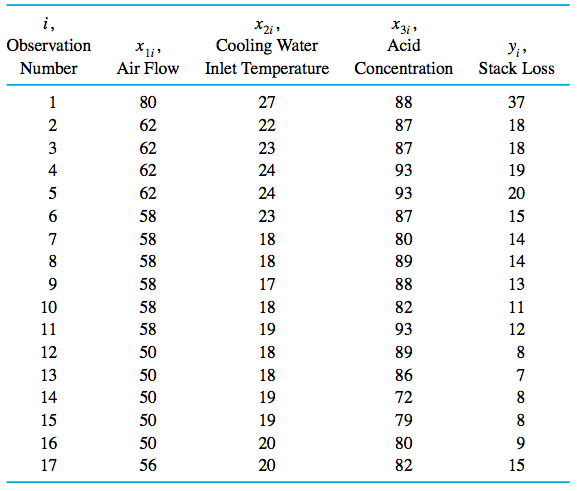
\includegraphics{../../fig/stack.png}
\end{frame}



\begin{frame}
\frametitle{Example: stack loss}
\begin{itemize}
\item Given:
\begin{itemize}
\pause \item $n = 17$
\pause \item $y$: stack loss of nitrogen from the chemical plant.
\pause \item $x_1$: air flow, the rate of operation of the plant
\pause \item $x_2$, inlet temperature of the cooling water
\pause \item $x_3$: (\% circulating acid - 50\% )$\times 10$
\end{itemize}
\pause \item We'll test the full model: 
\begin{align*}
Y_i = \beta_0 + \beta_1 x_{1, i} + \beta_2 x_{2, i} + \beta_3 x_{3, i} + \e_i
\end{align*}
\pause against the reduced model:
\begin{align*}
Y_i = \beta_0 + \e_i
\end{align*}
at $\alpha = 0.05$.
\end{itemize}
\end{frame}


\begin{frame}
\frametitle{Example: stack loss}
\begin{enumerate}[1. ]
\item 
\begin{itemize}
\item $H_0: \beta_1 = \beta_2 = \beta_3 = 0$
\pause \item Not all of the $\beta_i$'s are 0, $i = 1, 2, 3$.
\end{itemize}
\pause \item $\alpha = 0.05$
\pause \item The test statistic is:
\begin{align*}
F = \frac{SSR/(p-1)}{SSE/(n-p)} = \frac{MSR}{MSE}  \sim F_{p - 1, \ n - p}
\end{align*}
\pause Assume:
\begin{itemize}
\pause \item $H_0$ is true.
\pause \item The full model is valid with the $\e_i$'s iid N(0,$\sigma^2$)
\end{itemize}
Reject $H_0$ if $F > F_{p - 1,\ n - p,\ 1 - \alpha} = F_{4 - 1,\ 17 - 4,\ 1 - 0.05}  = F_{3, 13, 0.95} = 3.41$.
\end{enumerate}
\end{frame}


\begin{frame}
\frametitle{Example: stack loss} \scriptsize
\begin{enumerate}
\setcounter{enumi}{3}
\item In JMP, fit the full model and look at the {\bf ANOVA table}:
\begin{center}
\setkeys{Gin}{width=.7\textwidth} 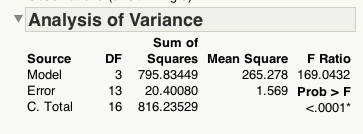
\includegraphics{../../fig/slfullanova1.png}
\end{center}
\pause by reading directly from the table, we can see: 
\begin{itemize}
\pause \item $p - 1 = 3$, $n - p = 13$, $n - 1 = 16$
\pause \item $SSR = 795.83, SSE = 20.4, SST = 816.24$
\pause \item $MSR = SSR/(p-1) = 795.83/3 = 265.28$
\pause \item $MSE = SSE/(n-p) = 20.4/13 = 1.57$
\pause \item $observed F = MSR/MSE = 265.78/1.57 = 169.04$
\pause \item Prob$>$F gives the p-value, $P( F_{3, 13} > observed F) < 0.0001$.
\end{itemize}
\pause \item With $F = 169.04 > 3.41$, we reject $H_0$ and conclude $H_a$.
\pause \item There is overwhelming evidence that at least one of air flow, inlet temperature, and \% circulating acid is important in explaining the variation in stack loss.
\end{enumerate}
\end{frame}

\begin{frame}
\frametitle{What if I want to compare different nested models?}
\begin{enumerate}[1. ]
\item 
\begin{itemize}
\item $H_0: \beta_{l_1}= \beta_{l_2}  = \cdots = \beta_{l_k} = 0$
\pause \item $H_a:$ not all of $\beta_{l_1}, \beta_{l_2}, \cdots, \beta_{l_k}$ are 0.
\pause \item 
(For example, $H_0: \beta_2 = \beta_3 = 0$ vs $H_a: \text{ either } \beta_2 \text{ or } \beta_3 \ne 0$ or both. The model is $Y_i = \beta_0 + \beta_1 x_{i,1} + \beta_2 x_{i,2} +  \beta_3 x_{i,3} +  \beta_4 x_{i,4} + \e_i$, and $k = 2$)

\end{itemize}
\pause \item $\alpha$ is some sensible value.
\pause \item The test statistic is:
\pause \begin{align*}
F = \frac{(SSR_f - SSR_r)/k}{SSE_f/(n-p)} \sim F_{k, \ n-p}
\end{align*}
\begin{itemize}
\pause \item $SSR_r$ is for the reduced model and $SSR_f$ is for the full model.
\pause \item Of course, we assume $H_0$ is true and the full model is valid with the $\e_i$'s iid $N(0, \sigma^2)$.
\end{itemize}
\end{enumerate}
\end{frame}


\begin{frame}
\frametitle{What if I want to compare different nested models?} \scriptsize
\begin{enumerate} 
\setcounter{enumi}{3}
\item We can construct a combined ANOVA table:
\begin{center}
\begin{tabular}{llllll}
Source & SS & df & MS & F & \\ \hline
Reg (full) & $SSR_f$ & $p-1$ &  & &  \\ 
Reg (reduced) & $SSR_r$ & $p-k-1$&  & &  \\ 
Reg (full $\mid$ red) & $SSR_f - SSR_r$ & $k$ & $\frac{SSR_f - SSR_r}{k}$ & $\frac{MSR_{f \mid r}}{MSE_f}$ &  \\ 
Error & $SSE_f$ & $n-p$ & $\frac{SSE_f}{n-p}$& & \\ \hline
Total & $SST$ & $n-1$ & & & 
\end{tabular}
\end{center}
\item 
Reject $H_0$ if observed F $> F_{p-1, n - p, 1 - \alpha}$. Or use the p-value: $P(F_{p-1, n-p} > observed F)$; reject $H_0$ when p-value is small.
\end{enumerate}
\end{frame}


\begin{frame}
\frametitle{Example: stack loss}
\begin{enumerate}[1. ]
\item 
\begin{itemize}
\item $H_0: \beta_2 = \beta_3 = 0$
\pause \item $H_a: $ either $\beta_2 \ne 0$ or $\beta_3 \ne 0$
\end{itemize}
\pause \item $\alpha = 0.05$
\pause \item The test statistic is:
\begin{align*}
\uncover<5->{F} & \uncover<5->{= \frac{(SSR_f - SSR_r)/k}{SSE_f/(n-p)}} \uncover<6->{= \frac{(SSR_f - SSR_r)/2}{SSE_f/(17 - 4)}} \\
& \uncover<7->{= \frac{(SSR_f - SSR_r)/2}{SSE_f/13}}
\end{align*}
\begin{itemize}
\uncover<8->{\item Assume $H_0$ is true and the full model is valid with the $\e_i$'s iid $N(0, \sigma^2)$.}
\uncover<9->{\item Then, $F \sim F_{k, \ n -p} = F_{2, 13}$.}
\uncover<10->{\item I will reject $H_0$ if $F > F_{2, 13, 0.95} = 3.81$.}
\end{itemize}
\end{enumerate}
\end{frame}

\begin{frame}
\frametitle{Example: stack loss} \small
\begin{enumerate}
\setcounter{enumi}{3}
\item Look at the ANOVA tables in JMP for both the full model ($Y_i = \beta_0 + \beta_1 x_{1, i} + \beta_2 x_{2, i} + \beta_3 x_{3, i} + \e_i$): 
\pause \begin{center}
\setkeys{Gin}{width=.7\textwidth} 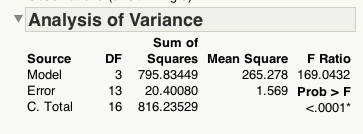
\includegraphics{../../fig/slfullanova1.png} 
\end{center}
\pause and the reduced model ($Y_i = \beta_0 + \beta_1 x_{1, i}  + \e_i$): 
\begin{center}
\setkeys{Gin}{width=.7\textwidth} 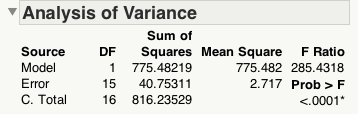
\includegraphics{../../fig/slredanova1.png}
\end{center}
\end{enumerate}
\end{frame}

\begin{frame}
\frametitle{Example: stack loss} \small
I construct a different ANOVA table for this test:
\begin{center}
\begin{tabular}{llllll}
Source & SS & df & MS & F & \\ \hline
Reg (full) & $ 795.83  $ & $4$ &  & &  \\ 
Reg (reduced) & $775.48$ & $2$&  & &  \\ 
Reg (full $\mid$ red) & $20.35$ & $2$ & $10.18$ & $6.48$ &  \\ 
Error & $20.4$ & $13$ & $1.57$& & \\ \hline
Total & $SST$ & $16$ & & & 
\end{tabular}
\end{center}
\begin{enumerate}
\setcounter{enumi}{4}
\pause \item With $observed F = 6.48 > 3.81$, I reject $H_0$ and conclude $H_a$.
\pause \item There is enough evidence to conclude that at least one of inlet temperature and \% circulating acid is associated with stack loss.
\end{enumerate}
\end{frame}

\begin{frame}
\frametitle{Example: stack loss}
\begin{itemize}
\item Attempt to eliminate inlet temperature ($x_2$) from the model at $\alpha = 0.05$. Here is the ANOVA table for the full model:
\begin{center}
\setkeys{Gin}{width=.7\textwidth} 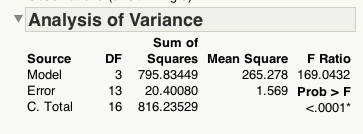
\includegraphics{../../fig/slfullanova1.png}
\end{center}
and for the reduced model:
\begin{center}
\setkeys{Gin}{width=.7\textwidth} 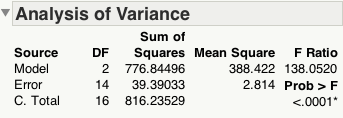
\includegraphics{../../fig/slredanova2.png}
\end{center}
\end{itemize}
\end{frame}


\begin{frame}
\frametitle{Example: stack loss}
\begin{enumerate}[1. ]
\item $H_0: \beta_2 = 0$, $H_a: \beta_2 \ne 0$
\pause \item $\alpha = 0.05$
\pause \item The test statistic is:
\begin{align*}
\uncover<4->{F} &\uncover<4->{= \frac{(SSR_f - SSR_r)/k}{SSE_f/(n-p)}}\uncover<5->{ = \frac{SSR_f - SSR_r}{SSE_f/(17 - 4)}} \\
& \uncover<6->{= \frac{SSR_f - SSR_r}{SSE_f/13}}
\end{align*}
\begin{itemize}
\uncover<7->{\item Assume $H_0$ is true and the full model is valid with the $\e_i$'s iid $N(0, \sigma^2)$.}
\uncover<8->{\item Then, $F \sim F_{k, \ n -p} = F_{1, 13}$.}
\uncover<9->{\item I will reject $H_0$ if $F > F_{1, 13, 0.95} = 4.67$.}
\end{itemize}
\end{enumerate}
\end{frame}

\begin{frame}
\frametitle{Example: stack loss}
\begin{enumerate}
\setcounter{enumi}{3}
\item I construct a different ANOVA table for this test:
\begin{center}
\pause \begin{tabular}{llllll}
Source & SS & df & MS & F & \\ \hline
Reg (full) & $ 795.83  $ & $4$ &  & &  \\ 
Reg (reduced) & $776.84$ & $3$&  & &  \\ 
Reg (full $\mid$ red) & $18.99$ & $1$ & $18.99$ & $12.10$ &  \\ 
Error & $20.4$ & $13$ & $1.57$& & \\ \hline
Total & $SST$ & $16$ & & & 
\end{tabular}
\end{center}
\pause \item With $observed F = 12.10 > 4.67$, we reject $H_0$.
\pause \item There is enough evidence to conclude that stack loss varies with inlet temperature.
\end{enumerate}
\end{frame}

\begin{frame}
\frametitle{Example: stack loss}
\begin{itemize}
\item The $F$ test for eliminating one parameter is analogous to the $t$ test from before:
\begin{center}
\setkeys{Gin}{width=.7\textwidth} 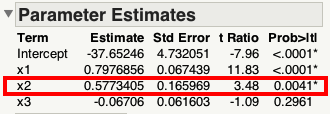
\includegraphics{../../fig/funfacttftest.png}
\end{center} 
\pause \item The t statistic for $H_0: \beta_2 = 0$ vs. $H_0: \beta_2 \ne 0$ is 3.48.
\pause \item But $3.48^2 = 12.1$, which is our $F$ statistic from the ANVOA test!
\pause \item Fun fact:
\begin{align*}
F_{1, \ \nu} = t_{\nu}^2
\end{align*}
\end{itemize}
\end{frame}


\subsection{The F test statistic and $R^2$}

\begin{frame}
\frametitle{The F test statistic and $R^2$}
\begin{itemize}
\item If $F$ is the test statistic from a test of $H_0: \beta_1 = \beta_2 = \cdots = \beta_{p - 1} = 0$ vs. $H_a:$ not all of $\beta_1, \beta_2, \ldots, \beta_{p-1}$ are 0, then $F$ can be expressed in terms of the coefficient of determination of the full model:
\pause \begin{align*}
F = \frac{R^2/(p-1)}{(1-R^2)/(n - p)}
\end{align*}
\pause \item For the stack loss example, the full model's $R^2$ = 0.975, and so:
\begin{align*}
F = \frac{0.975 / (4-1)}{(1-0.975)/(17-4)} = 169
\end{align*}
\end{itemize}
\end{frame}


\begin{frame}
\frametitle{The F test statistic and $R^2$}
\begin{center}
\setkeys{Gin}{width=.7\textwidth} 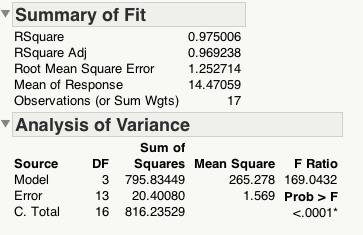
\includegraphics{../../fig/rsqf1.png}
\end{center}
\end{frame}

\begin{frame}
\frametitle{The F test statistic and $R^2$}
\begin{itemize}
\item For $H_0: \beta_1 = \beta_2 = \cdots = \beta_{p - 1} = 0$ vs. $H_a:$ not all of $\beta_1, \beta_2, \ldots, \beta_{p-1}$,
\end{itemize}
\begin{align*}
\uncover<2->{F} & \uncover<2->{= \frac{SSR \frac{1}{p-1}}{SSE\frac{1}{n-p}}} \uncover<3->{ = \frac{\frac{SSR}{SST} \frac{1}{p-1}}{\frac{SSE}{SST}\frac{1}{n-p}}} \uncover<4->{ = \frac{\frac{SSR}{SST} \frac{1}{p-1}}{\frac{SST - SSR}{SST}\frac{1}{n-p}}} \uncover<5->{ = \frac{\frac{SSR}{SST} \frac{1}{p-1}}{\left ( 1 - \frac{SSR}{SST} \right ) \frac{1}{n-p}}} \\
&\uncover<6->{= \frac{R^2 \frac{1}{p-1}}{(1- R^2) \frac{1}{n-p}}}
\end{align*}
\end{frame}

\begin{frame}
\frametitle{The F test statistic and $R^2$}
\begin{itemize}
\item If $F$ is the test statistic from a test of $H_0: \beta_{l_1} = \beta_{l_2} = \cdots = \beta_{l_k} = 0$ vs. $H_a:$ not all of $\beta_{l_1}, \beta_{l_2}, \ldots, \beta_{l_k}$ are 0, then $F$ can be expressed in terms of the coefficient of determination of the full model ($R^2_f$) and that of the reduced model ($R^2_r$):
\pause \begin{align*}
F = \frac{(R^2_f - R^2_r)/k}{(1-R_f^2)/(n - p)}
\end{align*}
\pause \item For the stack loss example when we tested $H_0: \beta_2 = \beta_3 = 0$, $R_f^2$ = 0.975 and $R^2_r = 0.95$.
\pause \begin{align*}
F = \frac{(0.975  - 0.95)/ 2}{(1-0.975)/(17-4)} = 6.50
\end{align*}
which is close to the test statistic of 6.48 that we calculated before.
\end{itemize}
\end{frame}

\begin{frame}
\frametitle{The F test statistic and $R^2$}
\begin{itemize}
\item When we tested $H_0: \beta_2 = 0$, $R^2_r$ was 0.9517, so:
\pause \begin{align*}
F = \frac{(0.975  - 0.9517)/ 1}{(1-0.975)/(17-4)} = 12.117
\end{align*}
\end{itemize}
\pause which is close to the test statistic of 12.10 that was calculated directly from the ANOVA table.
\end{frame}

\begin{frame}
\frametitle{The F test statistic and $R^2$}
\begin{align*}
F &= \frac{(SSR_f - SSR_r) \frac{1}{k}}{SSE_f \frac{1}{n-p}} \uncover<2->{= \frac{\frac{SSR_f - SSR_r}{SST} \frac{1}{k}}{\frac{SSE_f}{SST} \frac{1}{n-p}}} \uncover<3->{ = \frac{\left (\frac{SSR_f }{SST}- \frac{SSR_r}{SST} \right ) \frac{1}{k}}{\frac{SST - SSR_f}{SST} \frac{1}{n-p}}} \\
&\uncover<4->{= \frac{\left (\frac{SSR_f }{SST}- \frac{SSR_r}{SST} \right ) \frac{1}{k}}{ \left ( 1 - \frac{SSR_f}{SST} \right )  \frac{1}{n-p}}} \uncover<5->{ =  \frac{\left (R^2_f - R^2_r \right ) \frac{1}{k}}{(1 - R^2_f) \frac{1}{n-p}}}
\end{align*}
\end{frame}
\end{document}
